In this section will discuss any extra research done on the project.
in this section we will discuss the following:
\begin{enumerate}
    \item ADC
    \item Radio module
\end{enumerate}
\subsection{ADC}
The MCP3008 was not  available when ordering parts,Another  part for this was choosen which is the  DFR0553 which has the following:
\begin{enumerate}
    \item a supply voltages(VCC) of 3.3 to 5 v
    \item Analog signal  detection 0 to 5v
    \item 4 analog chanel's
    \item resolution of 16 bits
    \item Operating current of 3mA
\end{enumerate}
\subsection{Radio module}
for  this  section we want  to keep  the following in mind :
\begin{enumerate}
    \item We want a module that will send  and  received data
    \item we don't  want  an  expensive solution due  to wanting to  have  multiple nodes
    \item must we pick a standard? 
    \item what module has  an open source project on it 
    \item how do we  set up  a   mesh network with this 
\end{enumerate}
\subsubsection{Do we need a radio standard?}
Lets assume we communicate with two pi via wires  we know that an interference will occur when  we  commutation that is wireless
we can have multiple cases where interference can  occur these are  the following:
\begin{enumerate}
    \item the signal being reflected of objects such as  trees
    \item the signal can reach the  receiver due to an object blocking the antenna
    \item the signal isn't  power to be picked up by the receiver
\end{enumerate}
one essential part of this project is the  ability to have  our nodes have an address to set this up
from a communication preceptive we could develop this when there is open source project that has sorted out the routeing for  you.
only issue with this approach is if there is any issues that come from the open source project we will inheritthene
with this in mind the following standards were found
\begin{enumerate}
    \item LoRa
    \item Zigbee
    \item Sigfox
\end{enumerate}
In \cite{Wu_Liebeherr_2023} lora is used  that will organize sensor
data from all nodes in the spanning tree toward the root(laptop /PC) this can be show by the  following:
\begin{figure}[h!]
    \centering
    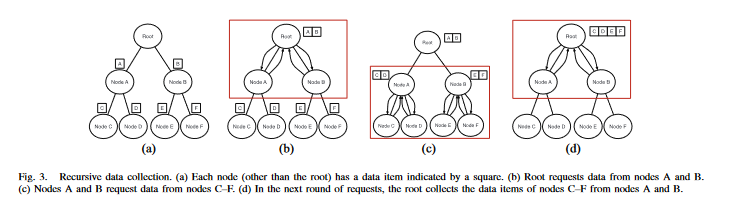
\includegraphics[width=0.5\linewidth]{Images/lora_example_routing_proto.png}
    \caption{protocol Wu used(wu\_lie et.al,2023:16705)}
    \label{protocol Wu used(wu_lie et.al,2023:16705)}
\end{figure}  
this proves it possible  to make a  mesh network using Lora.
\par 
from looking online Lora has more projects that are open source meaning we can use it.freely for example 
\par
for zigbee most of the application  that were found where indoor's i.e industial setting
  